\documentclass[11pt,a4paper]{article}
\usepackage{amsmath,amssymb}
\usepackage{graphicx}
\usepackage{hyperref}
\usepackage{geometry}
\usepackage{booktabs}
\geometry{margin=2.5cm}

\title{The Kitaev Chain: Dense BdG Implementation and\\
       Kernel Polynomial Method}
\author{}
\date{}

\begin{document}
\maketitle
\tableofcontents
\bigskip

% ─────────────────────────────────────────────────────────────────────────────
\section{The Kitaev Chain Model}
\label{sec:model}

The Kitaev chain~\cite{Kitaev2001} is the canonical one-dimensional model of a
spinless $p$-wave topological superconductor.  On a lattice of $N$ sites with
open boundary conditions (OBC) the Hamiltonian reads
\begin{equation}
  H = -t\sum_{i=1}^{N-1}\!\bigl(c_i^\dagger c_{i+1} + \mathrm{h.c.}\bigr)
      - \mu\sum_{i=1}^{N} c_i^\dagger c_i
      + \Delta\sum_{i=1}^{N-1}\!\bigl(c_i c_{i+1} + \mathrm{h.c.}\bigr),
  \label{eq:kitaev}
\end{equation}
where $t$ is the nearest-neighbour hopping, $\mu$ is the chemical potential,
and $\Delta \in \mathbb{R}$ is the $p$-wave pairing amplitude.
In the thermodynamic limit the bulk quasiparticle dispersion is
\begin{equation}
  E(k) = \pm\sqrt{\xi(k)^2 + \Delta^2\sin^2 k},
  \qquad \xi(k) = -2t\cos k - \mu,
\end{equation}
and the system is in the \emph{topological phase} for $|\mu| < 2t$, hosting a
pair of Majorana zero modes at the chain ends.  The topological phase
transition occurs at $|\mu| = 2t$.

\subsection{Bogoliubov–de Gennes (BdG) formulation}

To diagonalise~\eqref{eq:kitaev} one introduces the Nambu spinor
$\Psi_i = (c_i,\, c_i^\dagger)^T$ and writes the Hamiltonian in the
particle-hole doubled space.  The resulting $2N\times 2N$ BdG matrix is
\begin{equation}
  H_{\mathrm{BdG}} =
  \begin{pmatrix} H_{\mathrm{kin}} & \Delta A \\ \Delta A^\dagger & -H_{\mathrm{kin}} \end{pmatrix},
  \label{eq:BdG}
\end{equation}
where $H_{\mathrm{kin}}$ is the $N\times N$ OBC kinetic matrix,
\begin{equation}
  [H_{\mathrm{kin}}]_{ij} = -t\,(\delta_{i,j+1}+\delta_{i+1,j}) - \mu\,\delta_{ij},
\end{equation}
and $A$ is the nearest-neighbour pairing matrix with $A_{i+1,i}=1$ (OBC).
By particle-hole symmetry the spectrum of $H_{\mathrm{BdG}}$ is symmetric
about zero: if $E$ is an eigenvalue then so is $-E$.

\subsection{Dense matrix implementation}

The BdG matrix~\eqref{eq:BdG} is assembled directly in Julia as
\begin{verbatim}
H_kin = diagm(0 => fill(-mu, N), 1 => fill(-t, N-1), -1 => fill(-t, N-1))
A     = diagm(-1 => ones(N-1))
H_BdG = [H_kin  Delta*A; Delta*A'  -H_kin]
\end{verbatim}
The resulting $400\times 400$ matrix (for $N=200$) is shown in
Figure~\ref{fig:heatmap}.  The four blocks of~\eqref{eq:BdG} are clearly
visible: the tridiagonal kinetic blocks on the diagonal and the sparse pairing
blocks off-diagonal.

\begin{figure}[h]
  \centering
  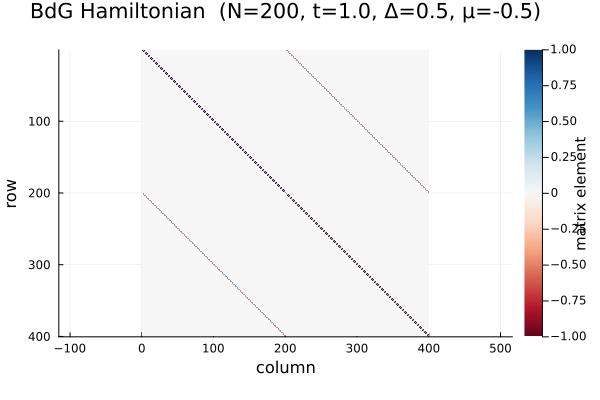
\includegraphics[width=0.65\textwidth]{figs/bdg_heatmap.png}
  \caption{Real part of the $2N\times 2N$ BdG Hamiltonian for $N=200$,
           $t=1$, $\Delta=0.5$, $\mu=-0.5$.  Red (positive) and blue
           (negative) entries reveal the block structure: diagonal kinetic
           blocks $\pm H_{\mathrm{kin}}$ and sparse off-diagonal pairing blocks
           $\Delta A$, $\Delta A^\dagger$.}
  \label{fig:heatmap}
\end{figure}

% ─────────────────────────────────────────────────────────────────────────────
\section{Kernel Polynomial Method}
\label{sec:kpm}

\subsection{Chebyshev expansion}

The Kernel Polynomial Method (KPM)~\cite{Weisse2006} approximates a spectral
function by expanding it in Chebyshev polynomials of the first kind,
$T_n(x) = \cos(n\arccos x)$, defined on $[-1,1]$.  Given the density of
states (DoS)
\begin{equation}
  \rho(\omega) = \sum_{i=1}^{d} \delta(\omega - \varepsilon_i),
\end{equation}
one first rescales the Hamiltonian to $\tilde H = (H - b)/a$ so that all
eigenvalues lie in $(-1,1)$, with
\begin{equation}
  b = \frac{E_{\max}+E_{\min}}{2}, \qquad
  a = \frac{E_{\max}-E_{\min}}{2}\times 1.1.
\end{equation}
The exact expansion of $\delta(E-\tilde H)$ in Chebyshev polynomials then
gives
\begin{equation}
  \rho(E) = \frac{1}{\pi\sqrt{1-E^2}}
  \Bigl[\mu_0 + 2\sum_{n=1}^{\infty} \mu_n\, T_n(E)\Bigr],
  \qquad \mu_n = \mathrm{tr}\!\left[T_n(\tilde H)\right].
  \label{eq:kpm_exact}
\end{equation}
Truncating to $N_{\mathrm{cheb}}$ terms and converting back to physical
energies $\omega = b + aE$ yields the approximation
\begin{equation}
  \rho(\omega) \approx
  \frac{1}{\pi\sqrt{1-E^2}\cdot N_{\mathrm{cheb}}\cdot a}
  \Bigl[\tilde g_0\,\mu_0 + 2\sum_{n=1}^{N_{\mathrm{cheb}}-1} \tilde g_n\,\mu_n\,T_n(E)\Bigr],
  \label{eq:kpm_trunc}
\end{equation}
where $\tilde g_n$ are the kernel damping weights (Section~\ref{sec:jackson}).

\subsection{Jackson kernel}
\label{sec:jackson}

The abrupt truncation of~\eqref{eq:kpm_exact} at order $N_{\mathrm{cheb}}$
introduces Gibbs oscillations.  The Jackson kernel suppresses them by
replacing the sharp cutoff with the smooth weights
\begin{equation}
  \tilde g_n = (N_{\mathrm{cheb}}-n)\cos\!\frac{\pi n}{N_{\mathrm{cheb}}}
              + \sin\!\frac{\pi n}{N_{\mathrm{cheb}}}\cot\!\frac{\pi}{N_{\mathrm{cheb}}},
  \qquad n = 0,\ldots,N_{\mathrm{cheb}}-1.
  \label{eq:jackson}
\end{equation}
Note that $\tilde g_0 = N_{\mathrm{cheb}}$ (unnormalized convention), which
accounts for the factor of $N_{\mathrm{cheb}}$ in the denominator
of~\eqref{eq:kpm_trunc}.  The effective energy resolution of the Jackson
kernel is $\delta E \sim \pi a / N_{\mathrm{cheb}}$.

\subsection{Chebyshev moment computation}

The moments $\mu_n = \mathrm{tr}[T_n(\tilde H)]$ are computed iteratively
using the three-term Chebyshev recurrence
\begin{equation}
  T_0(\tilde H) = I, \quad
  T_1(\tilde H) = \tilde H, \quad
  T_k(\tilde H) = 2\tilde H\,T_{k-1}(\tilde H) - T_{k-2}(\tilde H),
\end{equation}
storing only two matrices at a time and extracting the trace at each step.
The reconstruction of $\rho(\omega)$ at a given energy uses the same scalar
recurrence to evaluate $T_n(E)$ without storing polynomial matrices.

The resulting KPM density of states for the Kitaev chain is shown in
Figure~\ref{fig:dos_kpm}, with dashed lines marking the expected gap edges at
$\pm\Delta$.

\begin{figure}[h]
  \centering
  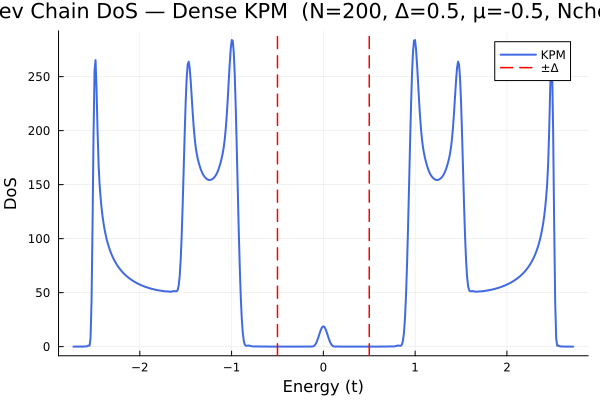
\includegraphics[width=0.65\textwidth]{figs/dos_kpm.png}
  \caption{KPM density of states of the Kitaev chain BdG Hamiltonian
           ($N=200$, $t=1$, $\Delta=0.5$, $\mu=-0.5$, $N_{\mathrm{cheb}}=200$).
           The gap of width $2\Delta$ around $\omega=0$ is characteristic of
           the topological phase.  Dashed red lines mark $\pm\Delta$.}
  \label{fig:dos_kpm}
\end{figure}

% ─────────────────────────────────────────────────────────────────────────────
\section{Comparison with Exact Diagonalisation}
\label{sec:comparison}

For a dense matrix of moderate size the full spectrum
$\{\varepsilon_i\}_{i=1}^{2N}$ is accessible via exact diagonalisation (ED).
A Lorentzian broadening of width $\eta$ replaces each delta function by
\begin{equation}
  \rho_{\mathrm{ED}}(\omega) = \sum_{i=1}^{2N}
  \frac{\eta}{\pi\!\left[(\omega-\varepsilon_i)^2+\eta^2\right]},
  \label{eq:lorentz}
\end{equation}
which integrates to $d = 2N$ (one contribution per eigenvalue), the same
convention as the KPM formula~\eqref{eq:kpm_trunc}.

The two approaches are compared in Figure~\ref{fig:comparison}.  The KPM
reproduces the peak positions and the spectral gap faithfully; the principal
differences are:
\begin{itemize}
  \item \textbf{Peak shape.}  The Jackson kernel broadens each delta function
        by $\sim\pi a/N_{\mathrm{cheb}}$, while the Lorentzian broadening is
        controlled by the explicit parameter $\eta$.  Setting
        $\eta \approx \pi a / N_{\mathrm{cheb}}$ makes the two
        representations broadly comparable.
  \item \textbf{Tails.}  Lorentzian tails decay as $\eta/\omega^2$, leading
        to spectral weight leaking into the gap region for finite $\eta$.
        The Jackson kernel has compact support in the rescaled variable $E$
        and produces sharper gap edges for the same effective resolution.
  \item \textbf{Scaling.}  KPM cost scales as $\mathcal{O}(N_{\mathrm{cheb}}\,d^2)$
        for a dense $d\times d$ matrix (matrix--matrix products), identical
        to the cost of building the Chebyshev expansion.  Full ED via
        \texttt{eigvals} costs $\mathcal{O}(d^3)$.  For large $d$ and
        moderate $N_{\mathrm{cheb}}$ the KPM becomes advantageous; for sparse
        matrices one can replace the matrix product by a matrix-vector product,
        reducing the cost to $\mathcal{O}(N_{\mathrm{cheb}}\,\mathrm{nnz})$.
\end{itemize}

\begin{figure}[h]
  \centering
  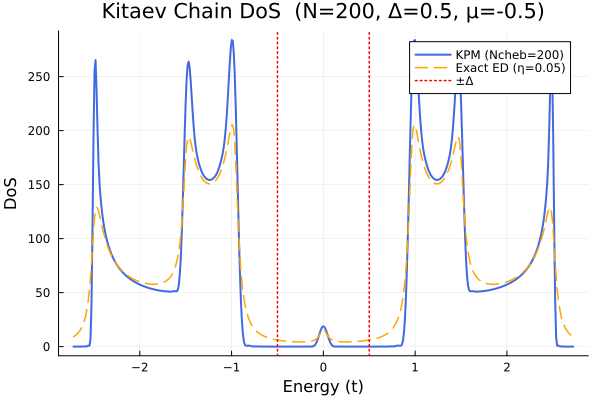
\includegraphics[width=0.65\textwidth]{figs/dos_comparison.png}
  \caption{Comparison of KPM ($N_{\mathrm{cheb}}=200$, blue) and
           Lorentzian-broadened exact ED ($\eta=0.05$, orange dashed) for the
           Kitaev chain DoS ($N=200$, $t=1$, $\Delta=0.5$, $\mu=-0.5$).
           Both curves are normalised so that $\int\rho\,d\omega = 2N$.
           Dotted red lines mark $\pm\Delta$.}
  \label{fig:comparison}
\end{figure}

% ─────────────────────────────────────────────────────────────────────────────
\begin{thebibliography}{9}
\bibitem{Kitaev2001}
  A.~Yu.~Kitaev,
  \emph{Unpaired Majorana fermions in quantum wires},
  Physics-Uspekhi \textbf{44}, 131 (2001).

\bibitem{Weisse2006}
  A.~Wei\ss{}e, G.~Wellein, A.~Alvermann, H.~Fehske,
  \emph{The kernel polynomial method},
  Rev.\ Mod.\ Phys.\ \textbf{78}, 275 (2006).
\end{thebibliography}

\end{document}
